\documentclass[aps,pra,twocolumn,reprint,floatfix,amsmath,amssymb]{revtex4-2}

\usepackage{graphicx}
\usepackage{booktabs}
\usepackage{siunitx}
\usepackage[colorlinks=true,linkcolor=blue,citecolor=blue,urlcolor=blue]{hyperref}
\usepackage{xcolor}
\usepackage{array}
\usepackage{mathtools}
\emergencystretch=2em

\begin{document}

\title{Native / Rich Multitone Feasibility for Ideal SQR and CPSQR}
\author{Codex}
\affiliation{Autonomous cQED Study Workspace}
\date{\today}

\begin{abstract}
This study asks the final patched-package version of a narrow control question: can multitone waveforms realize an ideal selective qubit rotation (SQR), and if not, can they at least realize a conditional-phase selective qubit rotation (CPSQR)? The workflow first audited the patched \texttt{cqed\_sim} conventions, then screened ten direct and composite waveform families on the harder \texttt{chi\_plus\_chiprime} model, retained five representative families, compared them across \texttt{chi\_only} and \texttt{chi\_plus\_chiprime} models, and finally refined duration thresholds for the most promising direct and echoed constructions. The central distinction is between reduced manifold-resolved qubit success and full joint qubit-cavity success. On reduced metrics, several direct and echoed families look excellent. On full joint metrics, the answer is much narrower: direct multitone can realize strict ideal SQR only on a restricted subset of the tested grid, while echoed/composite families do not rescue strict full-joint SQR. By contrast, echoed families realize the relaxed CPSQR target convincingly, often at essentially unit joint process fidelity and at shorter durations than the best strict-SQR cases. A key negative result is that high quartet validation on separate manifolds does not certify the joint operator: one echoed case reached strict reduced and full-state quartet means above $0.9999997$ while its strict joint process fidelity remained only $0.8677$. The scientifically honest conclusion is therefore mixed: strict ideal SQR is achievable only in limited direct cases, whereas CPSQR is the robust success notion for native/rich multitone echo constructions.
\end{abstract}

\maketitle

\section{Introduction}
Selective qubit rotations conditioned on cavity Fock number are a standard control primitive in dispersive circuit QED, where manifold-resolved transition frequencies arise naturally from the qubit-cavity interaction \cite{blais2021cqed,koch2007transmon}. In this workspace, the specific question has evolved through several narrower studies: some tested a single Gaussian multitone pulse against arbitrary block-diagonal qubit targets, some focused on residual-$Z$ suppression, some compared direct and echoed constructions, and some established that favorable single-input success is not enough. What remained missing was one final patched-package study that answered the clean question directly: can an ideal $x$-axis SQR be realized with native or richer multitone waveforms, and if not, can a weaker CPSQR target be realized instead?

This study answers that question using only the patched current \texttt{cqed\_sim} package \cite{cqedsim2026}. The design principle was to be scientifically conservative. We audited all patch-sensitive conventions before trusting earlier helpers or saved metrics, separated reduced and full-joint notions of success, included explicit negative controls, and treated echoed constructions as full physical sequences with finite inserted $X_\pi$ pulses rather than as idealized toggling-frame algebra. The result is not a blanket positive or negative claim. Instead, the answer depends sharply on the target notion and on whether one enforces the full joint qubit-cavity action.

\section{System and Methods}

\subsection{Hamiltonian}
The principal closed-system model is a two-level qubit dispersively coupled to a single cavity mode in the rotating frame used by the patched package audit. For the main grid we used
\begin{align}
\frac{H_0}{\hbar}
&=
\omega_c a^\dagger a
+
\omega_q |e\rangle\langle e|
\notag\\
&\quad+
\chi a^\dagger a\, |e\rangle\langle e|
\notag\\
&\quad+
\chi' a^\dagger a (a^\dagger a - 1)\, |e\rangle\langle e|
\notag\\
&\quad+
\frac{K}{2} a^{\dagger 2} a^2,
\label{eq:static_hamiltonian}
\end{align}
with $K=0$ in the principal grid. The \texttt{chi\_only} model sets $\chi'=0$, while the \texttt{chi\_plus\_chiprime} model uses the higher-order dispersive term retained by the patched package. In the qubit/cavity rotating frame $(\omega_q,\omega_c)$, the addressed manifold transition frequency is
\begin{align}
\Delta_n = \chi n + \chi' n(n-1).
\label{eq:manifold_frequency}
\end{align}

Within manifold $n$, a multitone drive produces an effective block Hamiltonian of the form
\begin{align}
\frac{H_n^{(\mathrm{eff})}(t)}{\hbar}
&=
\frac{\Omega_{x,n}(t)}{2} X
+
\frac{\Omega_{y,n}(t)}{2} Y
\notag\\
&\quad+
\frac{\Delta_n^{(\mathrm{ac})}(t)}{2} Z
+
H_{n,\mathrm{spec}}(t),
\label{eq:effective_block_hamiltonian}
\end{align}
where the first two terms are the desired transverse control, $\Delta_n^{(\mathrm{ac})}(t)$ is the manifold-dependent coherent $Z$ shift induced by simultaneous tones, and $H_{n,\mathrm{spec}}(t)$ collects spectator and off-resonant contributions. Equation~\eqref{eq:effective_block_hamiltonian} already explains why strict SQR is hard: the same waveform must fit all desired $\theta_n$ while suppressing manifold-dependent residual $Z$ structure.

\subsection{Simulation Parameters}
Table~\ref{tab:system_parameters} lists the parameters used in the main grid. The cavity truncation was chosen as $N_{\mathrm{cav}} = N_{\mathrm{active}} + 2$ so the addressed window could be checked for block preservation and redistribution into nearby spectator levels.

\begin{table}[t]
\centering
\caption{Main simulation parameters. The principal grid uses $n_{\mathrm{tr}}=2$, so higher-transmon leakage is intentionally excluded from the main answer.}
\label{tab:system_parameters}
\begin{tabular}{@{}lll@{}}
\toprule
Parameter & Value & Note \\
\midrule
$\omega_q/2\pi$ & \SI{6.150}{GHz} & qubit frequency \\
$\omega_c/2\pi$ & \SI{5.241}{GHz} & cavity frequency \\
$\chi/2\pi$ & \SI{-2.84}{MHz} & dispersive shift \\
$\chi'/2\pi$ & \SI{-21}{kHz} & higher-order dispersive term \\
$K/2\pi$ & \SI{0}{Hz} & cavity Kerr in main grid \\
$n_{\mathrm{tr}}$ & $2$ & principal grid \\
$N_{\mathrm{active}}$ & $2,3,4$ & addressed manifolds \\
$N_{\mathrm{cav}}$ & $N_{\mathrm{active}}+2$ & cavity truncation \\
$\Delta t$ & \SI{4}{ns} & solver time step \\
$\sigma/T$ & $1/6$ & Gaussian seed width \\
$T_{X_\pi}$ & \SI{40}{ns} & inserted echo pulse \\
\bottomrule
\end{tabular}
\end{table}

\subsection{Analytic Preliminary}
The strict target fixed throughout the study is
\begin{align}
U_{\mathrm{SQR}}^{\mathrm{ideal}}
=
\sum_{n\in\mathcal{A}} |n\rangle\langle n| \otimes R_x(\theta_n),
\label{eq:strict_target}
\end{align}
with addressed set $\mathcal{A}=\{0,\ldots,N_{\mathrm{active}}-1\}$ and $\phi_n=0$ so the target axis is strictly $\hat{x}$. The relaxed family is
\begin{align}
U_{\mathrm{CPSQR}}
=
\sum_{n\in\mathcal{A}} e^{i\gamma_n}|n\rangle\langle n| \otimes R_z(\delta_n)R_x(\theta_n).
\label{eq:cpsqr_target}
\end{align}
Strict ideal SQR is the special case $\gamma_n=\delta_n=0$ for all addressed $n$.

The perturbative direct-drive picture follows from Eq.~\eqref{eq:effective_block_hamiltonian}. The resonant tone at manifold $n$ sets the desired transverse angle $\theta_n$, while the other tones generate Stark-like shifts and coherent spectator terms. A direct multitone family therefore spends its degrees of freedom on two different jobs: matching the desired $\theta_n$ and canceling the accumulated
\begin{align}
\Phi_n \approx \int_0^T \Delta_n^{(\mathrm{ac})}(t)\,dt.
\label{eq:residual_phase}
\end{align}
This is why a weaker CPSQR family can remain reachable even when strict SQR fails: if the dominant mismatch is largely $\Phi_n$, allowing manifold-dependent post-rotation $Z$ phases removes the hardest constraint without changing the desired $x$-rotation angles.

For the echoed schedule
\begin{align}
\text{half-SQR} \rightarrow X_\pi \rightarrow \text{half-SQR} \rightarrow X_\pi,
\label{eq:echo_schedule}
\end{align}
ideal instantaneous and manifold-independent $X_\pi$ pulses would preserve the desired $X$ rotation while toggling $Z\mapsto -Z$, so the first-order residual phase in Eq.~\eqref{eq:residual_phase} would cancel for symmetric halves \cite{hahn1950echo}. The obstruction is physical rather than algebraic: the inserted $X_\pi$ pulses are themselves implemented on a dispersive ladder and are therefore not truly manifold independent. Once the refocusing pulse carries its own manifold dependence, the clean symmetry argument no longer guarantees strict ideal-SQR success.
\subsection{Computational Approach}
The patched convention audit covered \texttt{cqed\_sim.core.ideal\_gates}, \texttt{cqed\_sim.core.conventions}, \texttt{cqed\_sim.core.frequencies}, the relevant conditioned-multitone calibration modules, the sequence layer, and the physics convention report shipped with the package. Three upstream tests were re-run and passed:
\begin{enumerate}
    \item \path{tests/test_25_tensor_product_convention.py},
    \item \path{tests/test_23_sqr_additive_amplitude_correction.py},
    \item \path{tests/test_20_gaussian_iq_convention.py}.
\end{enumerate}
The audit confirmed the patched runtime convention used throughout this report:
\begin{enumerate}
    \item runtime tensor order is qubit $\otimes$ cavity;
    \item the flat Hilbert-space basis is qubit-major;
    \item the logical addressed ordering used for restricted operators is blockwise $(|g,0\rangle,|e,0\rangle,|g,1\rangle,|e,1\rangle,\ldots)$;
    \item \texttt{phi\_n} is an in-plane axis parameter, not a final Bloch azimuth;
    \item \texttt{fock\_fqs\_hz}, when overridden, is interpreted as an absolute transition-frequency override.
\end{enumerate}

The workflow had three numerical stages.
\begin{enumerate}
    \item \textbf{Screen}: ten families, twelve hard-model cases, and $120$ waveform-case evaluations on \texttt{chi\_plus\_chiprime}.
    \item \textbf{Comparison}: five retained families, forty-eight cases, and $240$ waveform-case evaluations across \texttt{chi\_only} and \texttt{chi\_plus\_chiprime}.
    \item \textbf{Duration refinement}: direct-family sweeps on $72$ cases plus a separate echoed sweep on $36$ cases.
\end{enumerate}

The screened families were:
\begin{enumerate}
    \item baseline Gaussian seed,
    \item native direct strict optimizer from the patched package,
    \item reduced-unitary direct re-optimization,
    \item symmetric two-segment direct envelope,
    \item complex-envelope direct family,
    \item basis-expanded direct family,
    \item fully symmetric echoed replay,
    \item independently corrected echoed family,
    \item weakly asymmetric echoed family,
    \item CPSQR-targeted echoed family.
\end{enumerate}
The screen retained five representative families for the final comparison: \texttt{gaussian\_seed}, \texttt{native\_direct\_strict}, \texttt{reduced\_unitary\_direct}, \texttt{echoed\_independent}, and \texttt{echoed\_asymmetric}.

Direct families were compared at fixed total multitone duration $T$. Composite families were compared at fixed active multitone duration $T$; their physical gate duration is $T+\SI{80}{ns}$ because of the two inserted \SI{40}{ns} $X_\pi$ pulses. The native direct family used the patched package's targeted-subspace optimizer. The study-local reduced-direct and echoed families used Powell optimization with bounded corrections and screen/comparison iteration caps of $18/26$ or $20/28$ depending on family complexity.

\subsection{Metrics}
The study separates three notions of success.

\paragraph{Reduced effective-qubit metrics.}
For each addressed manifold $n$, the full propagator defines a qubit channel $\mathcal{E}_n(\rho)=\sum_k K_{n,k}\rho K_{n,k}^\dagger$. The reduced process fidelity to a strict unitary target $U_n$ is
\begin{align}
F_n^{\mathrm{red}}(U_n,\mathcal{E}_n)
=
\frac{1}{4}\sum_k \left|\mathrm{Tr}(U_n^\dagger K_{n,k})\right|^2.
\label{eq:reduced_process}
\end{align}
Each manifold was also validated on the quartet $\{|g,n\rangle,|e,n\rangle,|+x,n\rangle,|+y,n\rangle\}$.

\paragraph{Full-state metrics.}
For the same quartet of initial states in each addressed manifold, we computed full-state fidelity to the strict and CPSQR targets, plus leakage outside the addressed window.

\paragraph{Full joint-unitary metrics.}
Restricting the full propagator to the addressed logical basis gives a $d\times d$ operator with $d=2N_{\mathrm{active}}$. The principal joint metric is
\begin{align}
F_{\mathrm{joint}}(U_{\mathrm{tgt}},U_{\mathrm{act}})
=
\frac{\left|\mathrm{Tr}(U_{\mathrm{tgt}}^\dagger U_{\mathrm{act}})\right|^2}{d^2}.
\label{eq:joint_process}
\end{align}
For strict SQR, $U_{\mathrm{tgt}}=U_{\mathrm{SQR}}^{\mathrm{ideal}}$. For CPSQR, $U_{\mathrm{tgt}}$ is built by fitting the best blockwise $\gamma_n$ and $\delta_n$ in Eq.~\eqref{eq:cpsqr_target}. We also report the operator-norm proxy $\lVert U_{\mathrm{act}}-U_{\mathrm{tgt}}\rVert_2$.

\section{Results}

\subsection{Direct Multitone Realizes Strict SQR Only on a Restricted Subset}
The screen already showed that the strongest strict-SQR performers were direct rather than composite families. Figure~\ref{fig:duration_strict} summarizes the median smooth-target trend for $N_{\mathrm{active}}\le 3$: direct families improve in both reduced and joint strict fidelity with increasing duration, whereas composite families improve strongly in reduced metrics but not in strict joint fidelity.

The best strict result on the comparison grid came from \texttt{reduced\_unitary\_direct} on the case \texttt{chi\_only\_smooth\_x\_na2\_chiT5p0}, with
\begin{align}
F_{\mathrm{joint}}^{\mathrm{strict}} = 0.998763,
\qquad
\lVert U_{\mathrm{act}}-U_{\mathrm{SQR}}^{\mathrm{ideal}}\rVert_2 = 0.0639.
\end{align}
This case also achieved a strict reduced quartet mean of $0.999414$, strict full quartet mean of $0.999414$, zero measurable addressed-window leakage, and a classification level of full ideal-SQR success.

However, the positive strict-SQR story does not generalize. Table~\ref{tab:thresholds} shows the refined duration thresholds for the best direct strict family, \texttt{reduced\_unitary\_direct}. Strict joint fidelity crossed $0.99$ at $|\chi|T/2\pi=3.0$ for \texttt{chi\_only} with $N_{\mathrm{active}}=2,3$ and for \texttt{chi\_plus\_chiprime} with $N_{\mathrm{active}}=2$. It never crossed $0.99$ for \texttt{chi\_plus\_chiprime}, $N_{\mathrm{active}}=3$, where the best refined value was only $0.984565$. On the broader comparison grid, all \texttt{chi\_plus\_chiprime}, $N_{\mathrm{active}}=4$ strict direct results remained below $0.95$. The correct conclusion is therefore conditional: direct multitone can realize strict ideal SQR, but only on the easier part of the tested space.

\begin{figure*}[t]
  \centering
  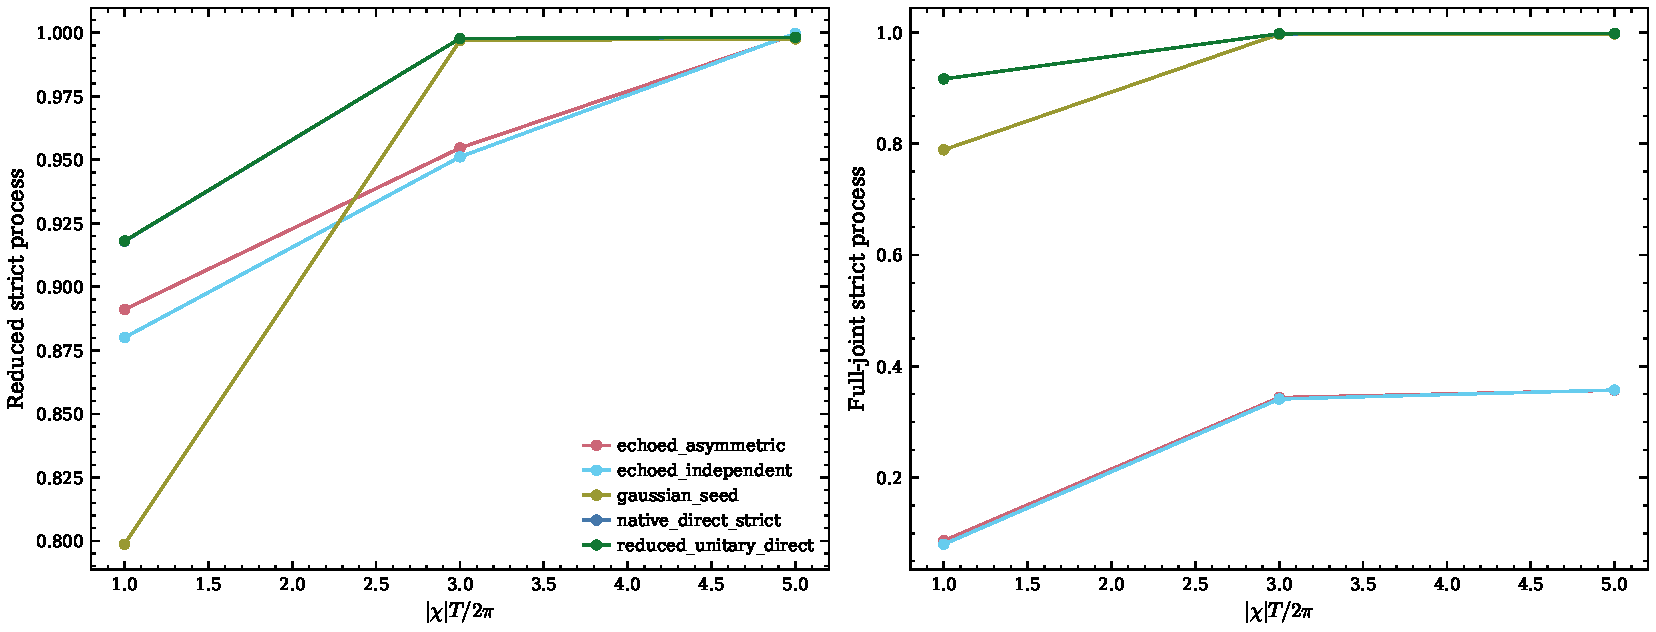
\includegraphics[width=\textwidth]{../figures/reduced_and_joint_fidelity_vs_duration.pdf}
  \caption{Median smooth-target performance for the five selected families and $N_{\mathrm{active}}\le 3$. Left: reduced strict process fidelity. Right: full-joint strict process fidelity. Direct families improve in both panels with duration, while composite families become much better on reduced metrics than on strict joint metrics.}
  \label{fig:duration_strict}
\end{figure*}

\subsection{Echo Helps CPSQR, Not Strict Full-Joint SQR}
The main positive result for composite control is not strict SQR but CPSQR. The clearest representative case is \texttt{echoed\_independent} on \texttt{chi\_plus\_chiprime\_staggered\_x\_na2\_chiT5p0}. For that pulse,
\begin{align}
F_{\mathrm{joint}}^{\mathrm{CPSQR}} &= 0.999999738, \\
F_{\mathrm{joint}}^{\mathrm{strict}} &= 0.867738, \\
\lVert U_{\mathrm{act}}-U_{\mathrm{CPSQR}}\rVert_2 &= 7.17\times 10^{-4}.
\end{align}
The per-manifold fitted residual phases were tiny: the fitted $\delta_n$ values were of order $10^{-4}$ to $10^{-3}$ rad and the mean residual-$Z$ error inside the fitted CPSQR blocks was only $3.74\times 10^{-4}$ rad. This is exactly the pattern predicted by the analytic preliminary: the echoed construction removes most of the coherent error relevant to Eq.~\eqref{eq:cpsqr_target}, but it does not restore the strict joint phase structure required by Eq.~\eqref{eq:strict_target}.

The echoed duration sweeps reinforce this interpretation. The best composite family, \texttt{echoed\_independent}, reached CPSQR joint fidelity above $0.99$ at $|\chi|T/2\pi=1.5$ for $N_{\mathrm{active}}=2$ and at $|\chi|T/2\pi=2.0$ for $N_{\mathrm{active}}=3$, under both \texttt{chi\_only} and \texttt{chi\_plus\_chiprime}. No echoed duration sweep reached strict joint fidelity above $0.99$. Figure~\ref{fig:direct_vs_echoed} shows the strict-joint comparison directly: the best composite construction remains far below the best direct construction on the strict objective across the refined duration axis.

\begin{figure}[t]
  \centering
  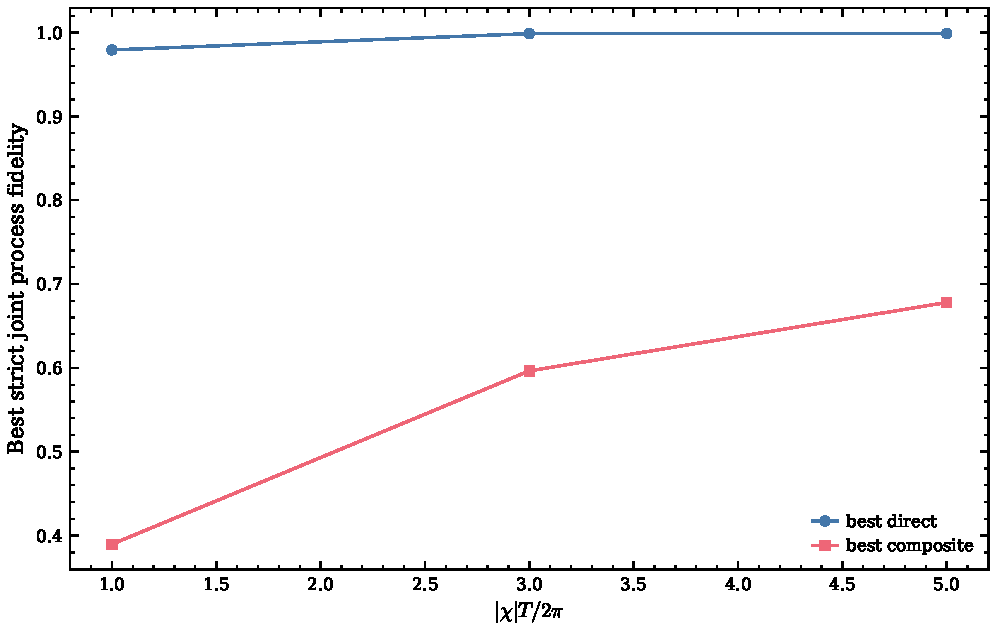
\includegraphics[width=\columnwidth]{../figures/direct_vs_echoed_comparison.pdf}
  \caption{Best strict full-joint process fidelity among direct families versus best strict full-joint process fidelity among composite families on the smooth-target structured subset. Composite control helps the relaxed CPSQR objective, but it does not overtake the best direct families on strict full-joint SQR.}
  \label{fig:direct_vs_echoed}
\end{figure}
\subsection{Reduced or Per-Input Success Does Not Certify the Joint Operator}
One of the user's central requirements was to answer the cavity-subspace question directly. The study therefore compared reduced metrics, full-state probe metrics, and the full joint operator on the same pulses. The most striking counterexample is again the best echoed CPSQR case. On that pulse, the strict reduced quartet mean was $0.999999737$ and the strict full-state quartet mean was $0.999999737$, yet the strict joint process fidelity was only $0.867738$. In other words, even excellent four-state validation inside each addressed manifold can miss the inter-manifold conditional phase structure that the full joint operator still gets wrong.

This observation sharpens the success hierarchy:
\begin{enumerate}
    \item reduced or even full-state manifold-wise success is not enough to claim strict SQR;
    \item the full joint operator is the decisive standard for the ``include cavity subspace'' version of the question;
    \item the echoed families are best interpreted as CPSQR realizations, not as strict joint SQR realizations.
\end{enumerate}
Figure~\ref{fig:sqr_vs_cpsqr} shows the family-level pattern. Direct families lie near the diagonal because their strict and CPSQR joint scores are similar when they work well. Composite families are displaced upward: their CPSQR joint fidelity is much higher than their strict joint fidelity, which is the signature of conditional-phase-dominated residual error.

\begin{figure}[t]
  \centering
  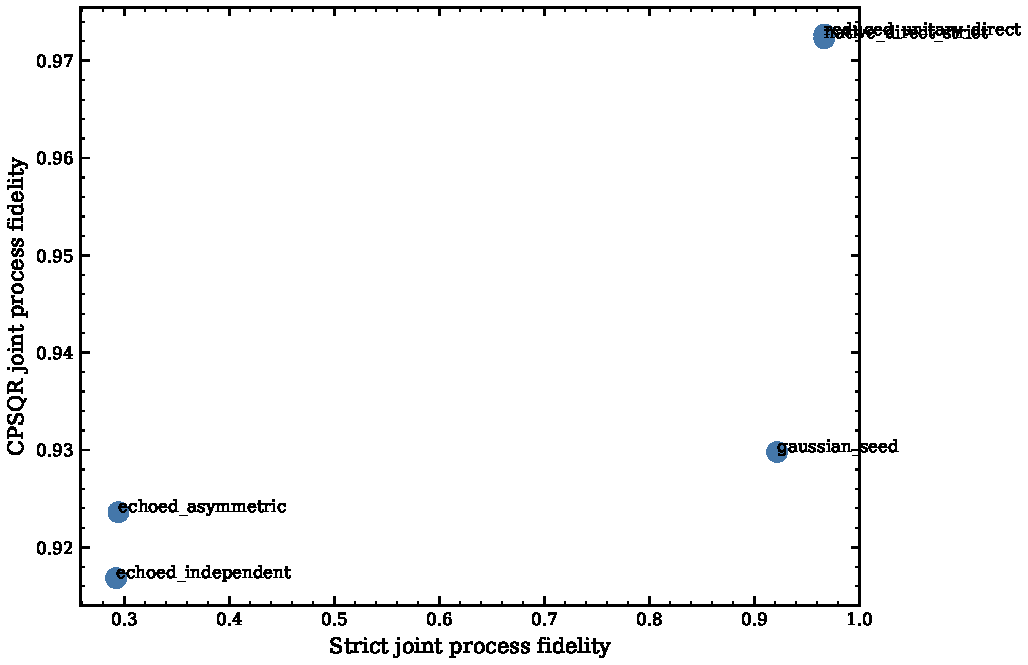
\includegraphics[width=\columnwidth]{../figures/sqr_vs_cpsqr_joint_comparison.pdf}
  \caption{Mean strict versus CPSQR joint process fidelity on the smooth-target structured subset with $N_{\mathrm{active}}\le 3$. Composite families cluster in the high-CPSQR/low-strict region, demonstrating that echo mainly converts the remaining error into conditional-phase structure rather than into full strict-SQR agreement.}
  \label{fig:sqr_vs_cpsqr}
\end{figure}

\subsection{Direct Answers to the Two Success Notions}
The question can now be answered in the two requested versions.

\paragraph{Version 1: Ignore the cavity subspace.}
If success is defined only by the manifold-resolved qubit action, then ideal-SQR-like behavior is common. Both strong direct families and several echoed families reached reduced quartet means above $0.99$, and the best echoed cases reached essentially perfect reduced strict and CPSQR scores.

\paragraph{Version 2: Enforce the full joint qubit-cavity operator.}
Under the full joint standard, the answer is much narrower. Strict ideal SQR survives only for a limited subset of direct multitone cases. Echoed constructions do not rescue strict joint SQR on the tested grids, but they do realize CPSQR convincingly. This distinction appears in the abstract, in Table~\ref{tab:main_answers}, and in the final conclusion.

\begin{table*}[t]
\centering
\caption{Direct answers to the study questions. ``Reduced-only'' ignores inter-manifold phase structure, while ``full-joint'' enforces the addressed joint qubit-cavity operator.}
\label{tab:main_answers}
\begin{tabular}{@{}llll@{}}
\toprule
Question & Reduced-only & Full-joint & Best family \\
\midrule
Direct strict SQR & Often yes & Limited subset only & \texttt{reduced\_unitary\_direct} \\
Echoed strict SQR & Often yes & No convincing success & \texttt{echoed\_independent} \\
Direct CPSQR & Yes & Yes on easy direct cases & \texttt{reduced\_unitary\_direct} \\
Echoed CPSQR & Yes & Yes, convincingly & \texttt{echoed\_independent} \\
Shortest duration & Short & CPSQR shorter than strict SQR & See Table~\ref{tab:thresholds} \\
\bottomrule
\end{tabular}
\end{table*}

\section{Validation}

\subsection{Sanity Checks}
The first validation layer was the convention audit itself. The patched tensor ordering, basis ordering, carrier sign convention, and \texttt{fock\_fqs\_hz} semantics were checked directly against the package source and tests. The audit also found a real stale-helper hazard: older study-local wrappers had passed frame-relative frequencies into a now absolute-frequency override. That mismatch was not used in the present workflow.

The second sanity layer was the legacy negative control. A representative saved pulse from an earlier study had a stored strict restricted-process fidelity of only $0.494918$. Replaying the same artifact under the patched current package gave
\begin{align}
F_{\mathrm{joint}}^{\mathrm{strict}} &= 0.824191, \\
\overline{F}_{\mathrm{quartet}}^{\mathrm{reduced}} &= 0.874684, \\
\overline{F}_{\mathrm{quartet}}^{\mathrm{full}} &= 0.874684.
\end{align}
This is strong evidence that old saved metrics could not be trusted blindly after the patch-sensitive convention changes.

\subsection{Convergence Analysis}
The direct and echoed duration refinements serve as the main convergence check. The key qualitative conclusions were stable across the two strongest direct families, \texttt{native\_direct\_strict} and \texttt{reduced\_unitary\_direct}: their threshold locations were effectively the same on the refined smooth-target grid. The strongest direct strict threshold appeared at $|\chi|T/2\pi=3.0$ for the easier regimes, and the harder \texttt{chi\_plus\_chiprime}, $N_{\mathrm{active}}=3$ regime consistently saturated below the $0.99$ strict-joint mark.

The echoed duration traces were not monotone in strict joint fidelity. That non-monotonicity is itself informative: it indicates that the improvement is not a clean symmetry-protected strict-SQR cancellation, but rather a fragile interplay between manifold-dependent halves and inserted finite $X_\pi$ pulses.

\subsection{Literature Comparison}
This study is not a paper-reproduction project, so there is no single external published benchmark for the exact patched-package target and metric stack. The closest applicable comparison is conceptual rather than numerical: the ideal echo logic of Hahn \cite{hahn1950echo} predicts first-order $Z$ cancellation only when the refocusing pulse is effectively manifold independent. The numerical results agree with that obstruction. The study also compared against prior internal claims through the patched negative-control replay, which is the right benchmark for this patch-sensitive workflow.

\section{Discussion}
The dominant error mechanism is now clear. When a waveform misses strict SQR but succeeds at CPSQR, the residual mismatch is mostly conditional phase structure rather than arbitrary transverse control failure. This is why the echoed families are so strong on Eq.~\eqref{eq:cpsqr_target}: they can make the manifold-resolved qubit map and even the per-input full-state evolution look nearly perfect while still missing the strict inter-manifold phase relations required by Eq.~\eqref{eq:strict_target}. The fact that one echoed pulse produced strict reduced and strict full-state quartet means above $0.9999997$ while still failing the joint strict metric by more than $0.13$ is the most direct numerical proof of that statement.

The direct families tell a different story. Because they do not insert additional manifold-dependent refocusing pulses, they can realize the strict joint operator cleanly on the easier regimes. The price is that they appear to run out of control freedom as the addressed set becomes harder, especially once the $\chi'$ term bends the manifold ladder through Eq.~\eqref{eq:manifold_frequency}. At that point, simultaneous fitting of the desired transverse angles and cancellation of manifold-dependent coherent phases becomes too constrained for the tested direct families.

The overall picture is therefore neither ``multitone works'' nor ``multitone fails.'' The truthful statement is more specific:
\begin{enumerate}
    \item direct multitone can realize strict ideal SQR on limited regimes;
    \item composite/echoed multitone does not rescue strict full-joint SQR;
    \item echoed multitone does realize CPSQR convincingly and often at shorter durations;
    \item reduced-only validation materially overestimates what survives full joint scrutiny.
\end{enumerate}

\section{Conclusion}
\begin{enumerate}
    \item \textbf{What is convincingly demonstrated:} direct multitone can realize strict ideal SQR on a restricted subset of the tested grid, while echoed multitone can realize CPSQR at essentially unit full-joint fidelity on multiple structured cases.
    \item \textbf{What is ruled out for the tested waveform classes:} a broad claim that native or modestly enriched multitone waveforms generically realize strict full-joint ideal SQR across the tested parameter space.
    \item \textbf{Whether strict ideal SQR is achievable:} yes, but only for limited direct cases; it is not established as a general property of the multitone family class.
    \item \textbf{Whether CPSQR is achievable:} yes, convincingly, and echoed constructions are especially effective for this relaxed target.
    \item \textbf{Whether success survives full-joint validation:} strict SQR survives only in limited direct cases; echoed successes mostly survive only as CPSQR, not as strict SQR.
    \item \textbf{What the current best waveform family is:} \texttt{reduced\_unitary\_direct} for strict SQR and \texttt{echoed\_independent} for CPSQR.
    \item \textbf{What the minimum convincing duration is:} for strict direct SQR, $|\chi|T/2\pi=3.0$ on the easier regimes; for echoed CPSQR, $|\chi|T/2\pi=1.5$ at $N_{\mathrm{active}}=2$ and $2.0$ at $N_{\mathrm{active}}=3$.
    \item \textbf{What the next most valuable follow-up is:} joint-phase-aware composite optimization together with $n_{\mathrm{tr}}=3$ sensitivity checks on the strongest strict and CPSQR cases.
\end{enumerate}

\section{Limitations and Future Work}
\subsection{Known Limitations}
The main grid is a closed-system $n_{\mathrm{tr}}=2$ study. This was intentional because the first goal was to settle the patched closed-system control question cleanly before adding higher-level leakage, cavity Kerr, or dissipation. The duration refinement was also focused on $N_{\mathrm{active}}=2,3$ and on the most informative smooth target, so the $N_{\mathrm{active}}=4$ strict answer rests on the comparison grid rather than on a dedicated duration sweep.

\subsection{Suggested Improvements}
\begin{itemize}
  \item \textbf{[P1 | MEDIUM]} Re-run the strongest strict-SQR and CPSQR cases with $n_{\mathrm{tr}}=3$ and verify whether the same hierarchy survives once explicit higher-level leakage is allowed.
  \item \textbf{[P1 | MEDIUM]} Optimize a composite family directly against the strict joint operator, including inter-manifold phase terms in the objective, to test whether the echoed strict failure is fundamental or merely an ansatz limitation.
  \item \textbf{[P2 | MEDIUM]} Add open-system follow-up for the best direct strict and best echoed CPSQR families only.
  \item \textbf{[P2 | LOW]} Upstream an explicit guard for the \texttt{fock\_fqs\_hz} absolute-frequency override so old frame-relative helpers cannot silently reappear.
\end{itemize}

\subsection{Open Questions}
The most important unresolved question is whether a composite family can preserve the echoed CPSQR benefit while also enforcing the missing inter-manifold strict phase structure. A second open question is whether the harder \texttt{chi\_plus\_chiprime}, $N_{\mathrm{active}}=3,4$ failures are genuinely control-limited or merely optimizer-limited.

\bibliographystyle{apsrev4-2}
\bibliography{references}

\appendix
\section{Detailed Results and Data}

\begin{table*}[t]
\centering
\caption{Minimum-duration summary for the strongest direct strict family (\texttt{reduced\_unitary\_direct}) and the strongest composite CPSQR family (\texttt{echoed\_independent}). ``Not reached'' means the threshold was not crossed on the refined duration grid.}
\label{tab:thresholds}
\resizebox{\textwidth}{!}{%
\begin{tabular}{@{}lllll@{}}
\toprule
Model & $N_{\mathrm{active}}$ & Direct strict $F_{\mathrm{joint}}\ge 0.99$ & Echoed CPSQR $F_{\mathrm{joint}}\ge 0.99$ & Interpretation \\
\midrule
\texttt{chi\_only} & 2 & $|\chi|T/2\pi = 3.0$ & $|\chi|T/2\pi = 1.5$ & CPSQR is faster than strict SQR \\
\texttt{chi\_only} & 3 & $|\chi|T/2\pi = 3.0$ & $|\chi|T/2\pi = 2.0$ & direct strict still viable, but slower \\
\texttt{chi\_plus\_chiprime} & 2 & $|\chi|T/2\pi = 3.0$ & $|\chi|T/2\pi = 1.5$ & similar easy-case hierarchy \\
\texttt{chi\_plus\_chiprime} & 3 & not reached (best $0.9846$) & $|\chi|T/2\pi = 2.0$ & strict direct fails, echoed CPSQR survives \\
\bottomrule
\end{tabular}
}
\end{table*}

\begin{table*}[t]
\centering
\caption{Representative optimized solutions used throughout the report. The strict solution is the global best strict-SQR case on the comparison grid. The echoed solution is the clearest CPSQR example with poor strict-joint fidelity on the same pulse.}
\label{tab:representative_cases}
\resizebox{\textwidth}{!}{%
\begin{tabular}{@{}llll@{}}
\toprule
Role & Family & Regime & Metrics \\
\midrule
Best strict SQR & \texttt{reduced\_unitary\_direct} & \texttt{chi\_only}, smooth\_x, $N_a=2$, $\chi T=5$ & strict $0.998763$, CPSQR $0.999647$ \\
Best CPSQR & \texttt{echoed\_independent} & \texttt{chi\_plus\_chiprime}, staggered\_x, $N_a=2$, $\chi T=5$ & strict $0.867738$, CPSQR $0.999999738$ \\
\bottomrule
\end{tabular}
}
\end{table*}

\begin{figure*}[t]
  \centering
  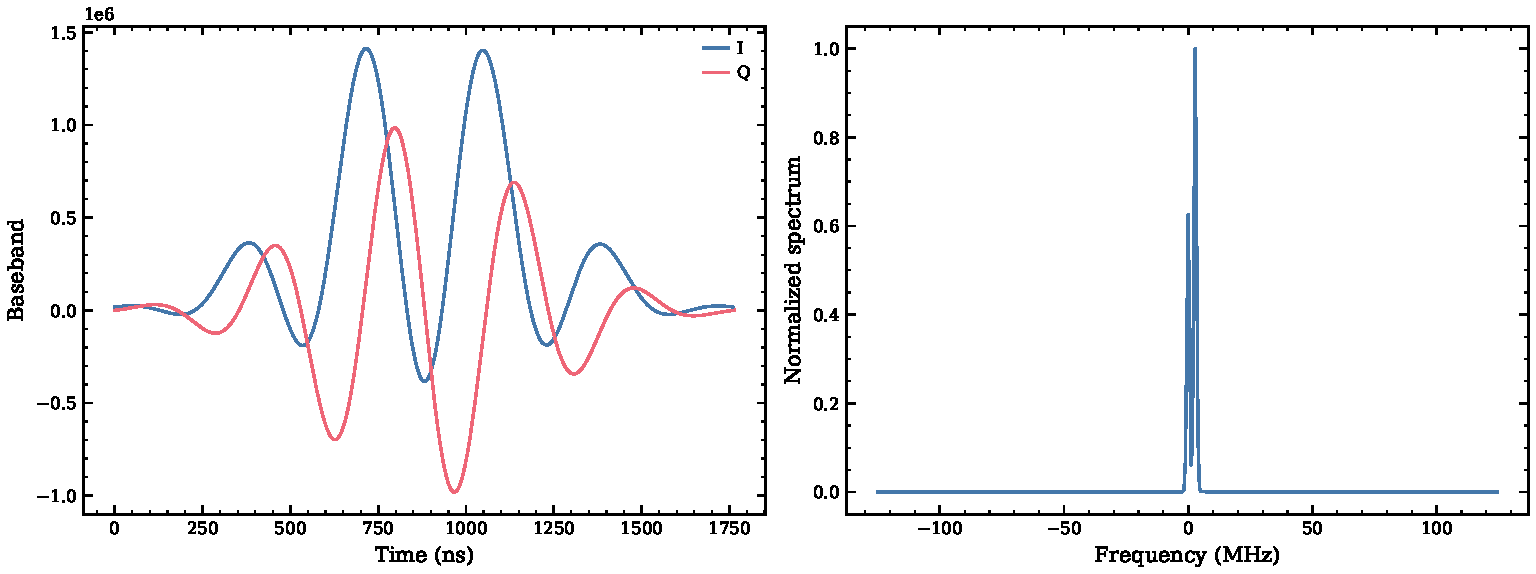
\includegraphics[width=\textwidth]{../figures/strict_best_waveform_and_spectrum.pdf}
  \caption{Representative best strict-SQR waveform. Left: baseband quadratures versus time. Right: normalized spectrum. This pulse corresponds to the direct family \texttt{reduced\_unitary\_direct} on \texttt{chi\_only\_smooth\_x\_na2\_chiT5p0}.}
  \label{fig:strict_waveform}
\end{figure*}

\begin{figure*}[t]
  \centering
  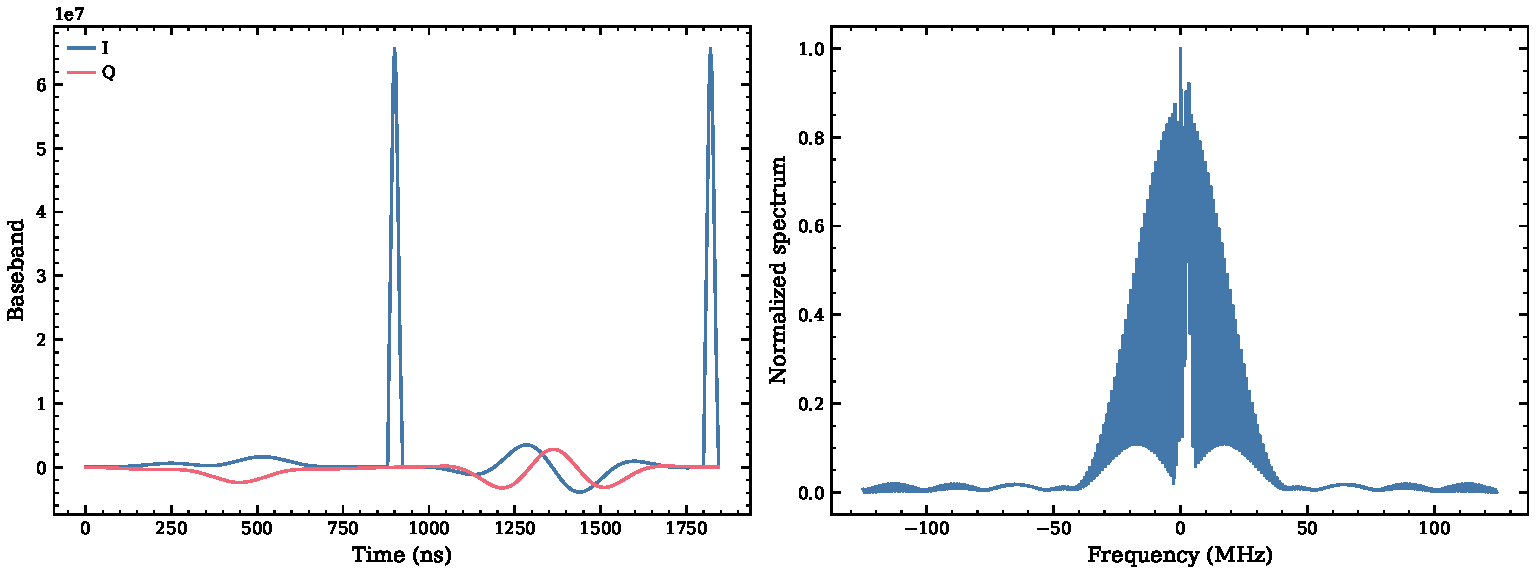
\includegraphics[width=\textwidth]{../figures/cpsqr_best_waveform_and_spectrum.pdf}
  \caption{Representative best CPSQR waveform. The plotted signal is the compiled echoed sequence whose active multitone duration is \SI{1760.56}{ns} and whose total gate duration is \SI{1840.56}{ns}.}
  \label{fig:cpsqr_waveform}
\end{figure*}

\begin{figure}[t]
  \centering
  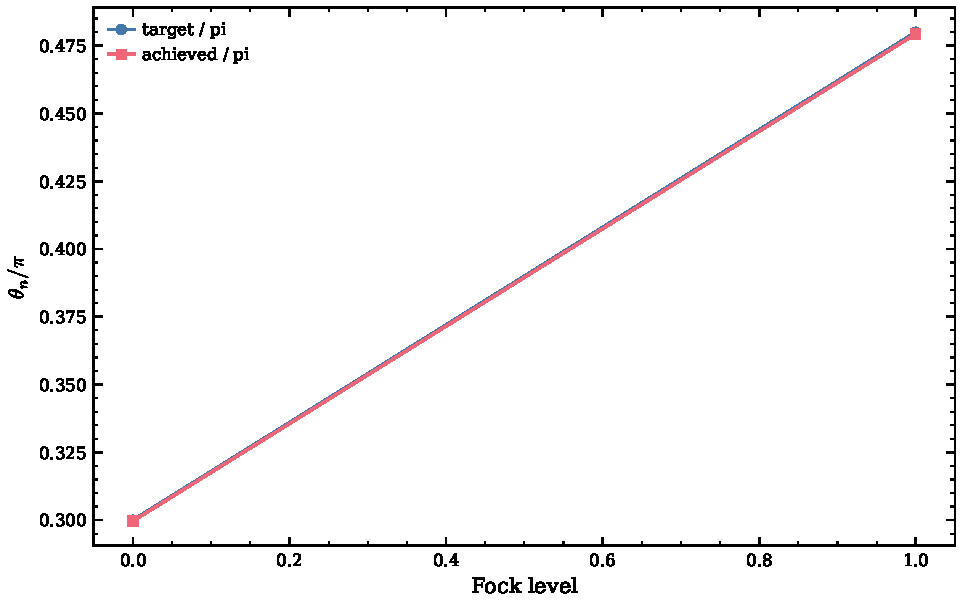
\includegraphics[width=\columnwidth]{../figures/strict_best_achieved_vs_target_angles.pdf}
  \caption{Target versus achieved rotation angles for the best strict direct solution.}
  \label{fig:strict_angles}
\end{figure}

\begin{figure}[t]
  \centering
  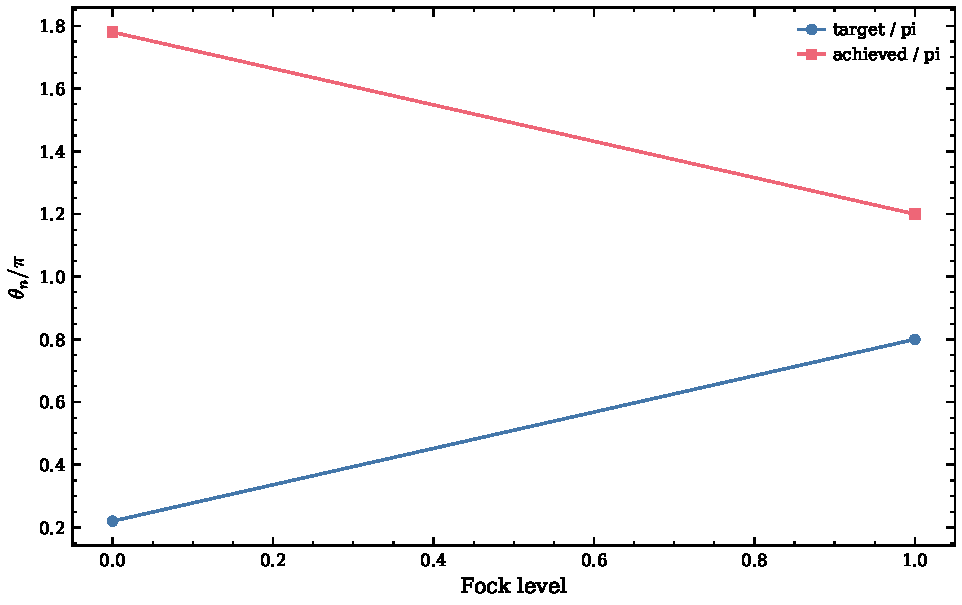
\includegraphics[width=\columnwidth]{../figures/cpsqr_best_achieved_vs_target_angles.pdf}
  \caption{Target versus achieved rotation angles for the representative echoed CPSQR solution after fitting the relaxed target family.}
  \label{fig:cpsqr_angles}
\end{figure}

\subsection{Optimized Parameters}
The best strict direct solution used the two corrected tones
\begin{align}
\delta\lambda &= (-7.35\times 10^{-5},\,-7.45\times 10^{-4}), \\
\delta\alpha &= (-5.56\times 10^{-5},\,-3.06\times 10^{-2}), \\
\delta\omega/2\pi &= (3.17\times 10^{-7},\,2.8400000000056275\times 10^{6})~\mathrm{Hz},
\end{align}
with tone amplitudes $(2.676\times 10^{5},\,4.276\times 10^{5})$ rad/s. The best echoed CPSQR solution used independent segment corrections:
\begin{align}
\delta\lambda^{(1)} &= (0.3362,\,-0.2038), &
\delta\lambda^{(2)} &= (-0.4699,\,0.6135), \\
\delta\alpha^{(1)} &= (-0.9507,\,2.9442), &
\delta\alpha^{(2)} &= (1.4069,\,-0.0377),
\end{align}
with equal segment durations of \SI{880.28}{ns} each and the two inserted \SI{40}{ns} $X_\pi$ pulses.

\subsection{Waveform and Pulse Information}
The strict direct waveform is a single multitone segment. The echoed CPSQR waveform is the four-pulse sequence in Eq.~\eqref{eq:echo_schedule}, with equal active halves and physical Gaussian $X_\pi$ pulses inserted between them. Publication figures for both waveforms are stored in \texttt{figures/} as both \texttt{.png} and \texttt{.pdf}. The machine-readable case artifacts store the sampled complex waveform arrays under \texttt{waveform\_samples}.

\subsection{Gate Sequence and Decomposition}
For the strict direct winner, the gate is one native multitone segment of total duration \SI{1760.56}{ns}. For the echoed CPSQR winner, the exact ordered sequence is:
\begin{enumerate}
    \item multitone half 1,
    \item Gaussian qubit $X_\pi$ pulse on the base channel,
    \item multitone half 2,
    \item Gaussian qubit $X_\pi$ pulse on the base channel.
\end{enumerate}
The two echoed halves are not identical; they are independently corrected, which is why the sequence achieves CPSQR but not strict symmetry-protected SQR.

\subsection{Modeling and Simulation Assumptions}
The principal study used $n_{\mathrm{tr}}=2$, $N_{\mathrm{cav}}=N_{\mathrm{active}}+2$, no dissipation, and $K=0$. The rotating frame was fixed at $(\omega_q,\omega_c)$, the addressed operator basis was blockwise $(|g,n\rangle,|e,n\rangle)$, and the integration step was \SI{4}{ns}. The main closure criterion for strict success was joint process fidelity above $0.99$ together with strong quartet validation.

\section{Reproducibility}

\subsection{Reproduction Procedure}
The study can be reproduced from the saved artifacts without re-running expensive optimizations:
\begin{enumerate}
    \item Open \path{scripts/reproducibility_notebook.ipynb}.
    \item Load the saved summary tables from \path{data/study_summary.json}, \path{data/comparison_results.json}, \path{data/duration_results.json}, and \path{data/duration_echoed_results.json}.
    \item Inspect the representative artifacts \path{artifacts/cases/chi_only_smooth_x_na2_chiT5p0_reduced_unitary_direct.json} and \path{artifacts/cases/chi_plus_chiprime_staggered_x_na2_chiT5p0_echoed_independent.json}.
    \item Re-generate the publication figures from the saved data.
    \item Optionally uncomment the re-run cells in the notebook to launch the corresponding single-case optimizations through the study scripts.
\end{enumerate}

\subsection{Saved Artifacts}
The primary machine-readable outputs are:
\begin{itemize}
    \item \path{data/study_summary.json}: executive summary, selected families, thresholds, representative rows.
    \item \path{data/comparison_results.json}: per-case comparison rows across all retained families.
    \item \path{data/duration_results.json}: refined direct-family duration sweeps.
    \item \path{data/duration_echoed_results.json}: refined echoed-family duration sweeps.
    \item \path{data/negative_controls.json}: patched replay of an old representative pulse.
    \item \path{data/study_results.csv}: flat combined table for all saved rows.
    \item \path{artifacts/cases/*.json}: per-case metrics, operators, probe-state tables, optimized parameters, and waveform samples.
    \item \path{figures/*.pdf} and \path{figures/*.png}: publication figures used in the report.
\end{itemize}

\subsection{Reproducibility Notebook}
The notebook exposes all tunable parameters in one early cell, rebuilds the model and derived objects from those parameters, defaults to loading saved results, and includes commented re-run cells for the representative direct strict and echoed CPSQR cases. The notebook is intended to be the fastest path for both users and future agents to verify the conclusions without re-reading the entire study history.

\end{document}
